\documentclass{book}
\usepackage[utf8]{inputenc}

\title{Space Systems Lab Firmware and Mission Requirements Document}
\author{Hersch Nathan}
\date{November 2024}

\usepackage{url}
\usepackage{float}
\usepackage{natbib}
\usepackage{graphicx}
\usepackage{listings}
\usepackage{fullpage}
\usepackage{hyperref}
\hypersetup{
    colorlinks=true,
    linkcolor=blue,
    filecolor=magenta,      
    urlcolor=cyan,
}

\begin{document}

\maketitle

\section{General Requirements}
\par This software is to support the KRUPS missions. The current mission is KRUPS Aboard Norwegian GhostSat (KANGS). The hardware paradim is based around an ESP32-S3. 
\par This work is porting Matt Ruffner's firmware for Adafruit Feather M0/M4 to the ESP32-S3. This including switching from the Arduino IDE to ESP-IDF.
\par The goal of this project is to make the firmware more modular and configurable for each mission and hardware.
\par The first chapter of this document outlines the overall architecture design and background information for this project. The second chapter provides information for writing firmware for this project. The third chapter details each library, driver, wrapper, and other software components that we wrote for this project. It provides design decisions and the reasoning behind them as well as how to interface with them. The fourth chapter and beyond detail the software requirements for each hardware component for each mission.

\tableofcontents

\chapter{Architechure Design} 
\section{Background Information}

\subsection{freeRTOS}
\par freeRTOS is a real time operating system. A real time operating system works by having tasks that run at different priorities. The tasks are scheduled by the operating system and those tasks occur through a determanistic prosess. The tasks can communicate with each other using message queues. The tasks can also synchronize with each other using semaphores.

\subsection{ESP-IDF}
\par ESP-IDF is the Espressif IoT Development Framework. It is the official development framework for the ESP32 and ESP32-S3. It is a set of libraries and tools that are used to develop software for the ESP32 and ESP32-S3.

\section{Overall Architecture Design}
\par The firmware's framework is designed to be modular and configerable thmission and each hardware. The backbone of the firmware is using freeRTOS tasks to handle the different modules. Each taks is its own module that encapsulates the relevant hardware. The tasks communicate with each other using a publisher/subscriber model.

\begin{figure} [H]
    \centering
    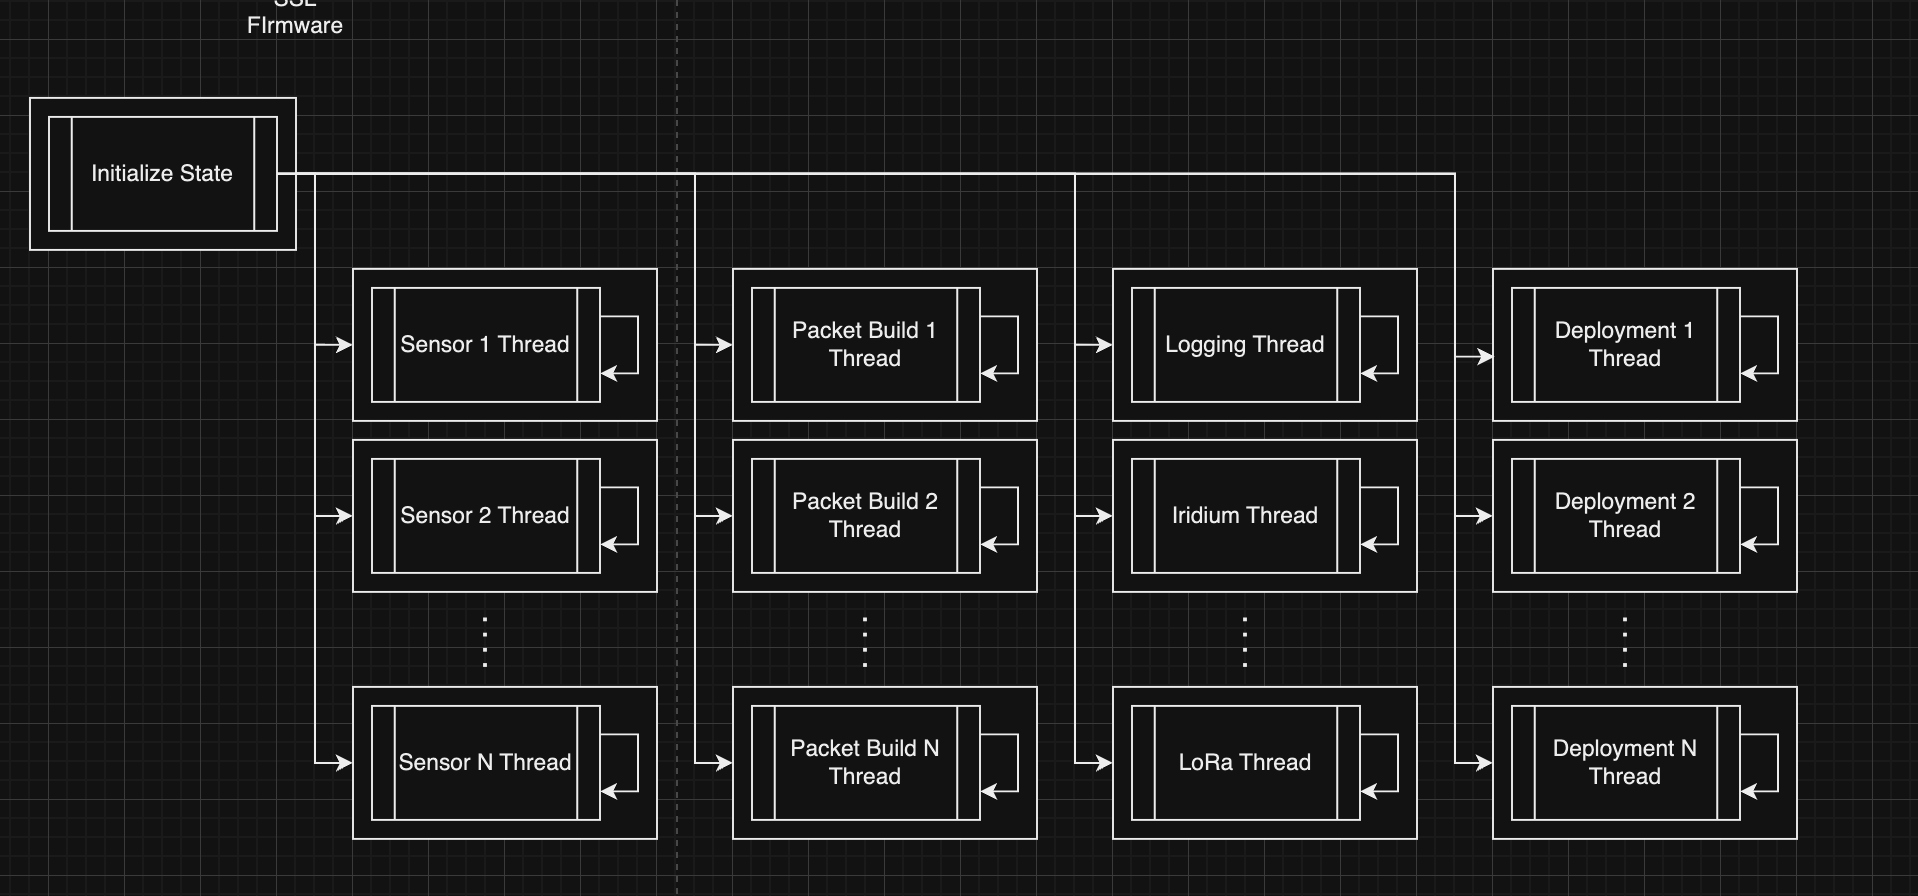
\includegraphics[width=0.8\textwidth]{images/firmware-architecture.png}
    \caption{Firmware Architecture}
    \label{fig:firmware-architecture} 
\end{figure}

\par In the figure \ref{fig:firmware-architecture}, the main tasks there are four types of tasks. 
\subsection{Task}
\subsubsection{Sensor Bus Tasks}
\par Each sensor bus task manages a single hardware bus (I2C, SPI, UART, etc). At startup, it configures the sensors with the necessary parameters, then it calls a looping task. That task takes the semaphore for the used serial communication interface. It sends the command to the sensor to get the data, reads the response, and then releases the semaphore. The task then sends the data to the packet build tasks queues.

\par The sensor manager works by creating a configuration for each bus, including the sensors connected to it, their intervals, and their handlers. It uses FreeRTOS timers to periodically trigger sensor events, which are added to a queue. The bus task processes these events, taking a mutex to ensure exclusive access to the bus, and calls the appropriate sensor handler from a lookup table. The handlers are responsible for reading data from the sensors and performing any necessary processing.

\begin{figure} [H]
    \centering
    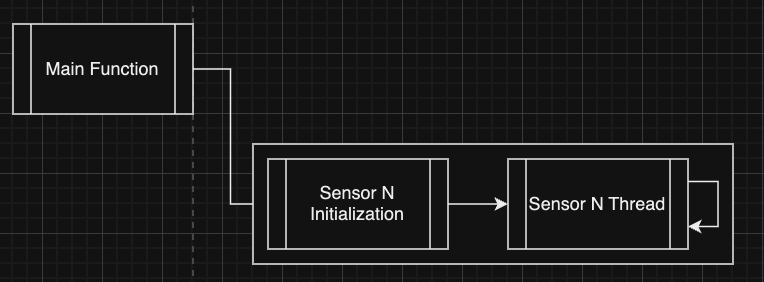
\includegraphics[width=0.15\textwidth]{images/sensor-architechure.png}
    \caption{Sensor Task Architecture}
    \label{fig:sensor-architecture} 
\end{figure} 

\subsubsection{Packet Build Tasks}
\subsubsection{Wireless Communication Tasks}
\subsubsection{Deployment Tasks}

\subsection{Middleware}



%%%%%%%%%%%%%%%%%%%%%%%%%%%%%%% Writing Firmware %%%%%%%%%%%%%%%%%%%%%%%%%
\chapter{Writing Firmware}

\section{Adding Components}

\par The current file stucture of SLLFirmware is as follows. It has 3 compoents the main firmware, the sensor drivers, and the manager drivers. If another compoent is to be added make sure to append it to the SSLFirmware/CMakeLists.txt file. Then create a folder for the component in the SSLFirmware folder. In that folder create a CMakeLists.txt file and the source files for the component. 

\begin{verbatim}
    SSLFirmware/
        - CMakeLists.txt
        - sdkconfig
        - main/
            - CMakeLists.txt
            - SSLFirmware.c
            - config.h
        - Manager/
            - i2c_manager/
                - CMakeLists.txt
                - i2c_manager.c
                - i2c_manager.h
        - Sensors/
            - CMakeLists.txt
            - BME280_Sensor/
                - CMakeLists.txt
                - BME280_Sensor.c
                - BME280_Sensor.h
                - BME280_API/
            - Fake_Sensor/
                - CMakeLists.txt
                - Fake_Sensor.c
                - Fake_Sensor.h
    \end{verbatim}

\par The CMakeLists.txt file for the project should look like the following. The EXTRA\_COMPONENT\_DIRS variable is used to add the components to the project. The include statement is used to include the project.cmake file from the ESP-IDF tools. The project name is set to SSLFirmware.

\begin{verbatim}
    cmake_minimum_required(VERSION 3.16)

    list(APPEND EXTRA_COMPONENT_DIRS ${CMAKE_SOURCE_DIR}/Manager)
    list(APPEND EXTRA_COMPONENT_DIRS ${CMAKE_SOURCE_DIR}/Sensors)

    include($ENV{IDF_PATH}/tools/cmake/project.cmake)

project(SSLFirmware)
\end{verbatim}

\par The CMakeList.txt file for each componet should look like the following. It specifies the source files for the component and the include directories for the component. The idf\_component\_register function is used to register the component with the project. The SRCS variable is used to specify the source files for the component. The INCLUDE\_DIRS variable is used to specify the include directories for the component. The PRIV\_REQUIRES variable is used to specify the components that the component requires. The REQUIRES variable is used to specify the components that the component depends on. 

\begin{verbatim}
    idf_component_register(SRCS "i2c_manager/i2c_manager" 
                            INCLUDE_DIRS "i2c_manager" 
                            PRIV_REQUIRES driver Sensors
                            REQUIRES main)
\end{verbatim}
%%%%%%%%%%%%%%%%%%%%%%%%%%%%%%% Software Componets %%%%%%%%%%%%%%%%%%%%%%%%%
\chapter{Software Components}
\section{Configuration}

\par To select the hardware that the firmware will use, use the menuconfig tool. To access the menuconfig tool, run the following command in the terminal. The options is under Hardware Configuration see figure \ref{fig:idfMenuconfig}. Then select the hardware that you want to use and save the configeration see figure \ref{fig:idfMenuconfig_hardware_options}. Later additions will have a selection for the mission then for each hardware component if this list gets too long.

\begin{center}
\noindent\fbox{%
    \parbox{\textwidth}{%
        \texttt{idf.py menuconfig}
    }%
}
\end{center}

\begin{figure} [H]
    \centering
    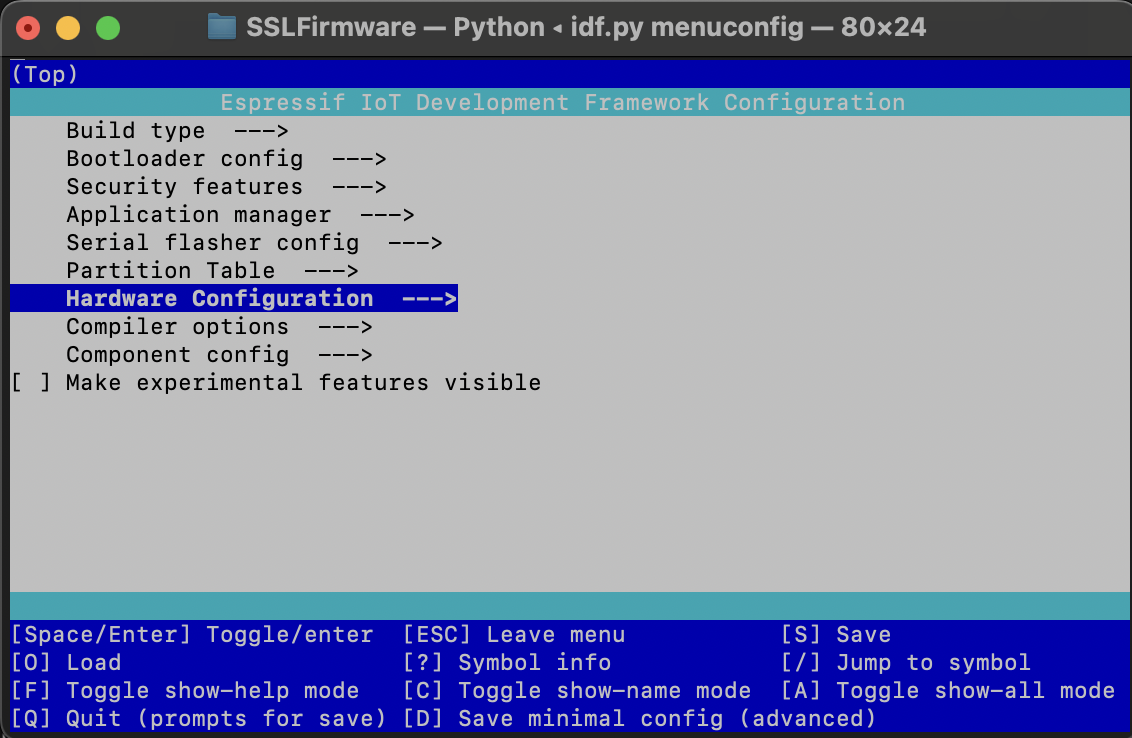
\includegraphics[width=0.8\textwidth]{images/idfMenuconfig.png}
    \caption{IDF Menuconfig}
    \label{fig:idfMenuconfig} 
\end{figure} 

\begin{figure} [H]
    \centering
    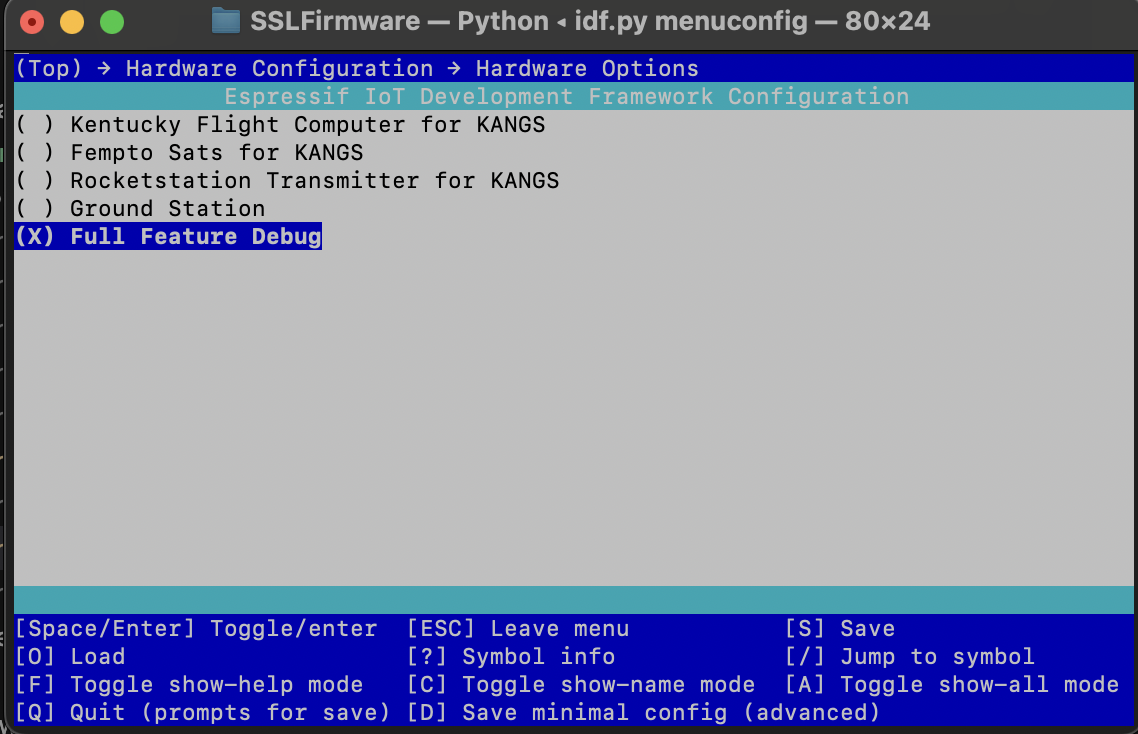
\includegraphics[width=0.8\textwidth]{images/idfMenuconfig_HardwareOptions.png}
    \caption{Hardware options}
    \label{fig:idfMenuconfig_hardware_options} 
\end{figure} 

\par the specific mission parameters (pinout, sensor configuration, etc) are set in the config.h file.



\section{Managers}

\subsection{I2C Manager}

\par The I2C manager is responsible for managing the I2C bus and interfacing with sensors connected to it. It provides a high-level interface for configuring sensors, setting up timers, and handling sensor events. The I2C manager is designed to be modular and extensible, allowing for easy integration of new sensors and bus configurations.

\par The I2C manager works as follows:
\begin{itemize}
    \item **Initialization**: The I2C manager initializes the I2C bus with the specified configurations. It sets up the I2C port, creates a queue for sensor events, and initializes a mutex for bus access control.
    \item **Sensor Configuration**: Before starting the timers, the I2C manager configures each sensor connected to the bus. This involves calling the sensor-specific configuration functions.
    \item **Timer Creation**: The I2C manager creates FreeRTOS timers for each sensor. These timers are set to trigger at specified intervals, defined in the sensor configuration. When a timer expires, it adds a sensor event to the event queue.
    \item **Event Handling**: The I2C manager runs a task that continuously waits for sensor events from the queue. When an event is received, it takes the mutex to gain exclusive access to the I2C bus, calls the appropriate sensor handler from the lookup table, and then releases the mutex.
\end{itemize}

\par Note that the timeout ticks are hard-defined to 1000 in the I2C manager header file. This value can be adjusted based on the specific requirements of the application.

\par The `i2cBusTask` is created as follows:

\begin{itemize}
    \item **I2CBusConfig**: This structure is used to configure the I2C bus. It includes the I2C port, sensor events, sensor intervals, sensor configuration functions, and the number of sensors. For example:
    \begin{verbatim}
    I2CBusConfig bus1Config = {
        .i2cPort = I2C_NUM_0,
        .sensorEvents = {SENSOR1_EVENT, SENSOR2_EVENT},
        .sensorIntervals = {sensorIntervals[SENSOR1_EVENT], sensorIntervals[SENSOR2_EVENT]},
        .sensorConfigs = {SENSOR1_config, SENSOR2_config},
        .sensorCount = 2
    };
    \end{verbatim}
    \item **Event Queue**: An event queue is created for each I2C bus to hold sensor events. This queue is used to pass events from the timers to the I2C bus task. For example:
    \begin{verbatim}
    bus1Config.eventQueue = xQueueCreate(10, sizeof(SensorEventType));
    \end{verbatim}
    \item **Mutex**: A mutex is created for each I2C bus to ensure exclusive access to the bus. This prevents conflicts when multiple tasks try to access the bus simultaneously. For example:
    \begin{verbatim}
    bus1Config.mutex = xSemaphoreCreateMutex();
    \end{verbatim}
    \item **Task Creation**: The `i2cBusTask` is created using the `xTaskCreate` function. This function takes the task function, task name, stack size, task parameters, task priority, and task handle as arguments. For example:
    \begin{verbatim}
    xTaskCreate(i2cBusTask, "I2CBusTask1", 2048, &bus1Config, 5, NULL);
    \end{verbatim}
\end{itemize}

%%%%%%%%%%%%%%%%%%%%%%%%%%%%%%% Missions %%%%%%%%%%%%%%%%%%%%%%%%%
\chapter{KRUPS Aboard Norwegian GhostSat (KANG)}
\section{Kentucky Flight Computer (KFC) Requirements}

\section{FemptoSats Requirements}
\par The FemptoSats submission is to test the viability of using Wifi/LoRa for intercapsuole communication. 

\subsection{Sensors Requirements}
\par The FemptoSats will have the following sensors: 
\begin{itemize}
    \item BME280 Temperature/pressure/humidity sensor
    \item BNO086 9 - Axis IMU
\end{itemize}

\subsubsection{BME280 Temperature/pressure/humidity sensor}
\par The BME280 will be run with the following configuration settings: 

\subsubsection{BNO086 9 - Axis IMU}
\par The BNO086 will be run with the following configuration settings:

\subsection{Wireless Communcation Requirements}
\par The FemptoSat will use the following Wireless Communication modules:
\begin{itemize}
    \item Integrated Wifi
    \item LoRa
\end{itemize}
\par The Wifi will fail over to the LoRa when the Wifi gets out of range

\section{Rocketstation Transmitter (RST) Requirements}
\par uart to raspi to shut off need

\subsection{Sensors Requirements}
\par The Rocketstation will have the following sensors: 
\begin{itemize}
    \item BME280 Temperature/pressure/humidity sensor
    \item BNO086 9 - Axis IMU
\end{itemize}

\subsubsection{BME280 Temperature/pressure/humidity sensor}
\par The BME280 will be run with the following configuration settings: 

\subsubsection{BNO086 9 - Axis IMU}
\par The BNO086 will be run with the following configuration settings:

\subsection{Wireless Communication Requirements}
\par The Rocketstation will use the following wireless Communication modules:
\begin{itemize}
    \item Integrated WiFi
    \item LoRa
\end{itemize}
\par The Wifi will fail over to the LoRa when the WiFi gets out of range. Communications between Rocketstation and FemptoSats will start once the satellites are deployed

\section{Rocketstation Requirements}
\par uart to raspi to shut off need
\section{Groundstation Requirements}




%\appendix

%\newpage
%\section{Arduino Pin Mapping}
%\label{app:pinmap}
%\lstinputlisting[language={}]{arduino-pinmap.txt}

%\bibliographystyle{plain}
%\bibliography{references}
\end{document}
